% UniTrackFormer: End-to-End TrackML Particle Tracking with Transformer
\documentclass{beamer}
\usepackage{graphicx}
\usepackage{tikz}
\usetikzlibrary{positioning}
\usetheme{Madrid}

\title{UniTrackFormer: End-to-End TrackML Particle Tracking with Transformer}
\author{Ivan Tang}
\date{May 2025}

\begin{document}

\begin{frame}
  \titlepage
\end{frame}

% Project Overview
\begin{frame}{Project Overview}
  \begin{itemize}
    \item \textbf{Goal:} End-to-end particle track reconstruction for the TrackML Challenge using deep learning.
    \item \textbf{Core Idea:} Use Transformer architecture to cluster detector hits into physical tracks.
    \item \textbf{Key Contributions:}
    \begin{itemize}
      \item End-to-end modeling, no manual feature engineering
      \item Multi-task loss: classification, clustering, and parameter regression
      \item Rich visualization and evaluation
    \end{itemize}
  \end{itemize}
\end{frame}

% Data Structure
\begin{frame}{Data Structure}
  \textbf{TrackML Raw Data:}
  \begin{itemize}
    \item \texttt{hits.csv}: Each hit's spatial coordinates (x, y, z), module info, etc.
    \item \texttt{truth.csv}: True particle ID (particle\_id) for each hit
    \item \texttt{detectors.csv}: Detector geometry info
  \end{itemize}
  \vspace{0.5em}
  \textbf{Feature Example:}
  \begin{center}
    \includegraphics[width=0.7\textwidth]{../../results/3d_hits.png}
  \end{center}
\end{frame}

% Data Table Example
\begin{frame}{Data Table Example}
  \begin{table}[]
    \centering
    \begin{tabular}{cccccc}
      \hline
      hit\_id & x & y & z & volume\_id & module\_id \\
      \hline
      1 & 123.4 & -56.7 & 789.0 & 8 & 12 \\
      2 & 234.5 & -67.8 & 800.1 & 8 & 13 \\
      ... & ... & ... & ... & ... & ... \\
      \hline
    \end{tabular}
    \caption{Sample fields from hits.csv}
  \end{table}
\end{frame}

% filepath: /Users/IvanTang/machinelearning/trackML/report/latex/main.tex
% Model Architecture
\begin{frame}{Model Architecture: UniTrackFormer}
  \begin{columns}[T,onlytextwidth]
    \column{0.52\textwidth}
      \vspace{0.2cm}
      \begin{itemize}
        \item \textbf{Input:} $N_{hits} \times D$ features
        \item \textbf{Encoder:} Multi-layer Transformer Encoder
        \item \textbf{Query:} $Q$ learnable query vectors
        \item \textbf{Decoder:} Multi-layer Transformer Decoder
        \item \textbf{Output:}
        \begin{itemize}
          \item Track classification
          \item Hit assignment (clustering)
          \item Parameter regression
        \end{itemize}
      \end{itemize}
    \column{0.48\textwidth}
      \begin{center}
      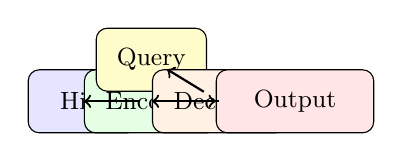
\begin{tikzpicture}[scale=0.48, every node/.style={font=\small}]
        % Nodes with absolute positions and more compact layout
        \node[draw, rounded corners, fill=blue!10, minimum width=1.4cm, minimum height=0.8cm] (input) at (0,0) {Hits};
        \node[draw, rounded corners, fill=green!10, minimum width=1.7cm, minimum height=0.8cm] (enc) at (1.8,0) {Encoder};
        \node[draw, rounded corners, fill=yellow!20, minimum width=1.4cm, minimum height=0.8cm] (query) at (1.8,1.1) {Query};
        \node[draw, rounded corners, fill=orange!10, minimum width=1.7cm, minimum height=0.8cm] (dec) at (3.6,0) {Decoder};
        \node[draw, rounded corners, fill=red!10, minimum width=2.0cm, minimum height=0.8cm] (out) at (5.6,0) {Output};

        % Arrows
        \draw[->, thick] (input) -- (enc);
        \draw[->, thick] (enc) -- (dec);
        \draw[->, thick] (query) -- (dec);
        \draw[->, thick] (dec) -- (out);
      \end{tikzpicture}
      \end{center}
  \end{columns}
\end{frame}

% Multi-task Loss
\begin{frame}{Multi-task Loss}
  \begin{itemize}
    \item \textbf{Track classification loss} (Binary Cross Entropy)
    \item \textbf{Mask clustering loss} (Dice + BCE)
    \item \textbf{Physical parameter regression loss} (MSE)
    \item Total loss = $\alpha$ classification + $\beta$ mask + $\gamma$ params
  \end{itemize}
\end{frame}

% Training and Evaluation
\begin{frame}{Training and Evaluation}
  \begin{enumerate}
    \item Data loading and feature extraction
    \item Model training (supports K-fold cross-validation)
    \item Evaluation metrics: efficiency, fake rate
    \item Visualization: 3D distribution, rz projection, track clustering
  \end{enumerate}
  \begin{center}
    \includegraphics[width=0.5\textwidth]{../../checkpoints/loss_curve.png}
  \end{center}
\end{frame}

% Visualization Results
\begin{frame}{Visualization Results}
  \begin{columns}
    \column{0.5\textwidth}
      \includegraphics[width=\textwidth]{../../results/ground_truth.png}
      \centering Ground Truth Tracks
    \column{0.5\textwidth}
      \includegraphics[width=\textwidth]{../../results/predictions.png}
      \centering Predicted Tracks
  \end{columns}
\end{frame}

% Summary
\begin{frame}{Summary and Outlook}
  \begin{itemize}
    \item End-to-end TrackML tracking pipeline implemented
    \item Multi-task loss and rich visualization supported
    \item Future: optimize model, improve clustering, enhance physics interpretability
  \end{itemize}
  \vspace{1em}
  \centering
  \textbf{Thank you! Questions welcome.}
\end{frame}

\end{document}